%************************************************************************************
% Authors: Martin Nordio
% Date: March 2011
% Root file: report_root.tex
%************************************************************************************


%----------------------------------------------------------------------------
\chapter{Implementation}\label{implementation}
%----------------------------------------------------------------------------



\section{Introduction}

CloudStudio consists of three distinct implementation parts at this point: the server, the client and the web interface. The server and client are both written in Java, while the web interface runs in JavaScript. \\

The client periodically sends data to the server to keep the awareness information of CloudStudio up to date. The server provides a public API to request awareness information directly, as well as a user-friendly web interface that uses and showcases the full capabilities of the API. \\

The server provides a central login system for its users and allows them to work with Git repositories hosted independently from CloudStudio. \\

A MySQL database stores all of the data; its details are explained in section \ref{database}.





\section{Architecture}

\subsection{Architectural Overview}

While in \ref{designapproach} the entire system was presented from a global point of view, this section deals with the internal architecture of CloudStudio system. Figure \ref{fig:entities} shows an architectural overview of all entities in CloudStudio. \\

\begin{figure}[h!]
  \centering
      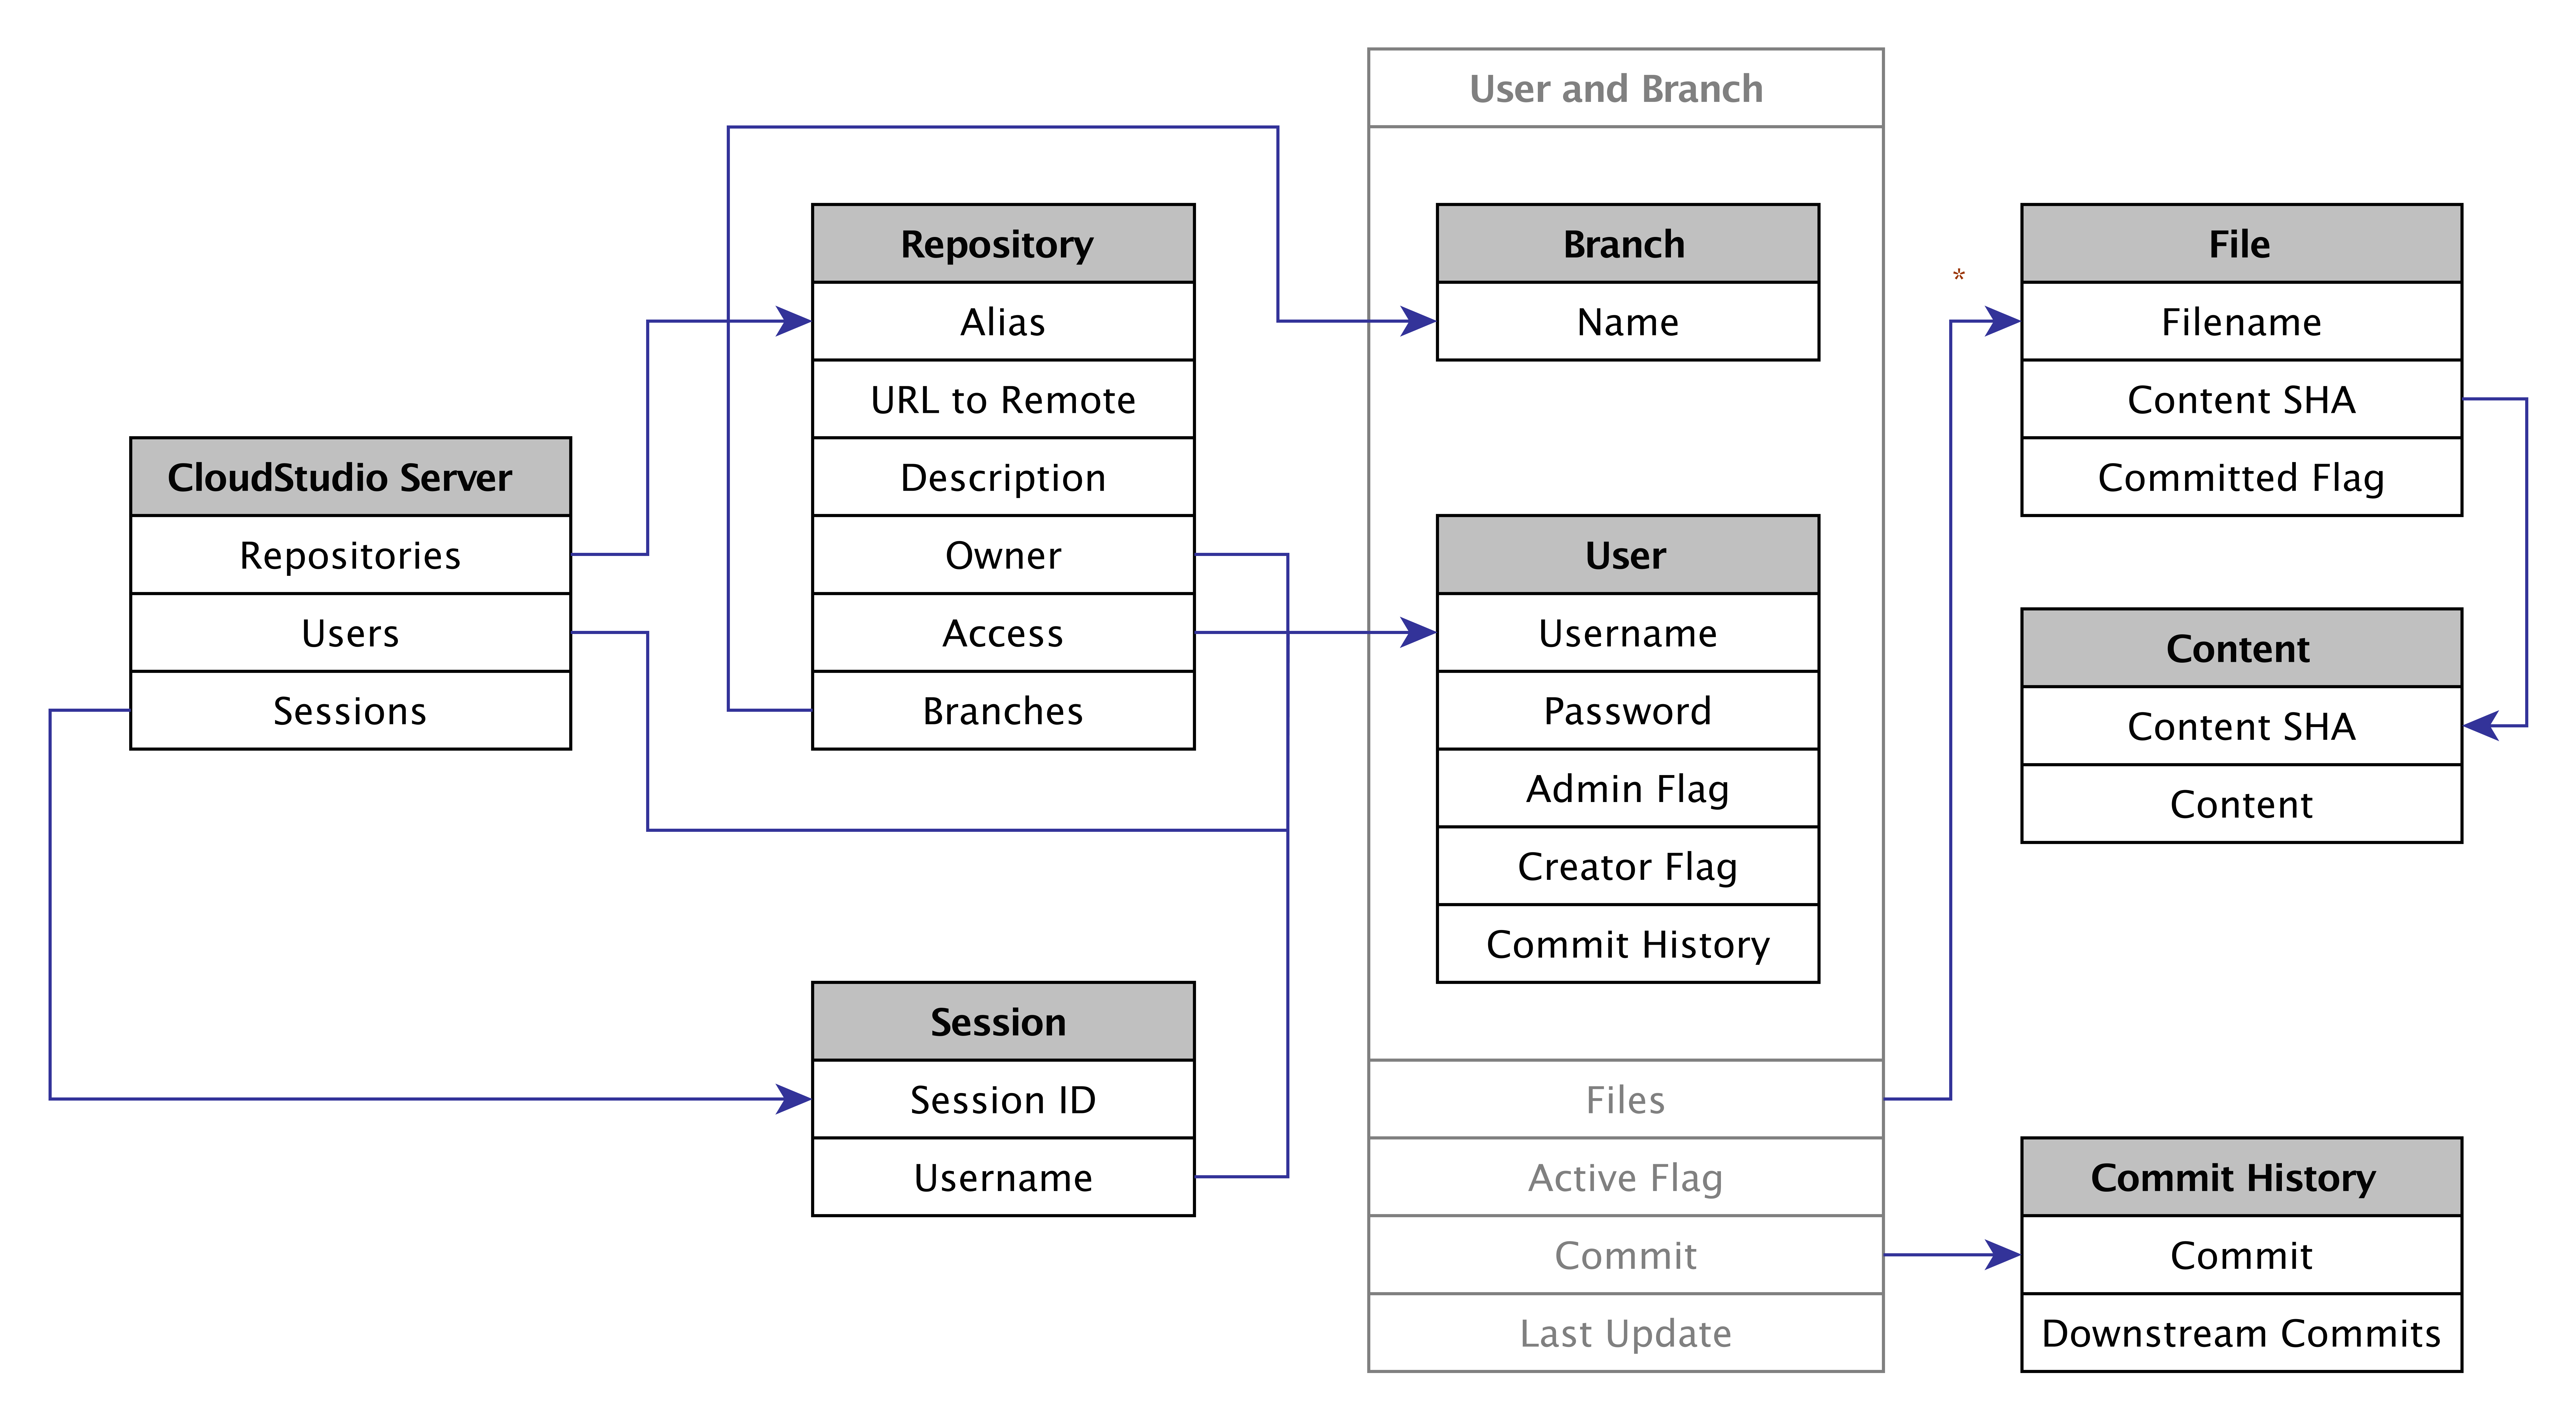
\includegraphics[width=1\textwidth]{entities}
  \caption{CloudStudio architecture}
  \label{fig:entities}
\end{figure}


The CloudStudio server primarily knows about users, repositories and sessions. \\

In order to do any sort of data manipulation or awareness requests, a user needs to request a session ID from the server via the $login$ API routine. This session ID will then be sent in every subsequent request to the server to verify a user's authentication. A new user can also be created using the $createUser$ API command. \\

A user has a username, a password (that is hashed before storing it), an admin flag (determines whether a user has administrator privileges) and a creator flag (indicating the ability of a user to create new repositories). \\

Repositories refer to the internal CloudStudio entity of a shared Git repository. A repository has an alias (its internal and unique name in CloudStudio), a description, a URL to a remote repository (e.g. on GitHub), a list of users that have access to it and an owner (who can modify repository specific data, add or remove users, or delete the repository entirely). \\

For every user and branch in the repository, the information sent by the CloudStudio client is stored individually. On the level of a single repository, this means that every user has one or several branches that contain files, a (partial) commit graph, an active flag (indicating whether a user has currently checked out this branch into his working tree) and a timestamp when the user has last sent information about this branch to the CloudStudio server. \\

Files are represented as an object with a filename, a content SHA checksum and a $committed$ value. The $committed$ value can be one of three values: $committed$ (this exact file is currently part of a local commit), $uncommitted$ (this is the latest version of a file directly from the working directory) or $both$ (the uncommitted and committed files and contents are identical in this branch). \\

All of the above information is stored in the MySQL database, while the content of the files are stored in the filesystem, named by their SHA. The file object points to its content via the SHA. \\

A special user named "origin" is automatically added to the server and every repository and represents the central remote repository. It stores the Git information the same way a normal CloudStudio user would.

\subsection{Logic}

One of the key parts to note here is that CloudStudio stores branch and file information for each user and repository separately. Aggregated awareness information is prepared by the server at the time it is requested by the respective API call. \\

The server does not directly store a combined commit history but only a partial history for every user. More specifically, for every branch in a repository, the transitive set of parent commits of the current branch commit is stored in a list, internally named $downstream$ $commits$. To find the nearest common ancestor commit to calculate a merge conflict, we can simply go through the list of downstream commits of two users and choose the one with the smallest combined distance from the respective branch commit. \\

Every CloudStudio repository can have a central remote Git repository URL attached. CloudStudio needs to fetch its information regularily for two main reasons:

\begin{enumerate}
\item Retrieving the commit graph in order to find the relative position for the branch awareness view.
\item The CloudStudio client only sends commit data (such as files and their content) for commits that have a local branch reference point to them. For conflict detection, files in the merge-base commit are directly looked up from the origin through JGit. Since we assume that users synchronise their repositories through the specified remote repository, this always works, because the merge-base commit necessarily needs to have been pushed to the origin at some point.
\end{enumerate}

As much of the logic as possible has been implemented directly as SQL queries, which positively affects the performance. This works especially well for branch and file awareness. For content awareness, a lot of calculations are performed directly in Java: file contents need to be looked up through JGit and comparison is implemented using the respective diff and diff3 algorithms.

\subsection{Access Control}

CloudStudio provides a central login structure, which can be used by many users collaborating on different shared projects. Each repository has a designated owner who has the rights to add or remove people to the project, change its metadata, elect a new owner, or remove the repository altogether. \\

Administrators can manage users and their privileges, as well as perform any actions that a repository owner or normal user could. A "creator" flag for each user indicates whether or not they have the privilege to create new repositories on CloudStudio. In the server configuration, you can enable or disable to set this flag by default for new users. In some closed environments, e.g. teachers set up projects for students and add them to the project, it may be preferred that not all users can create new repositories on CloudStudio.


\subsection{Folder Structure}

The source files are divided into 4 folders at the root level: $CSClient$ contains the client classes, $CSServer$ contains the server classes and the web interface, $CSCommon$ contains classes shared by client and server, and $CSTesting$ contains the JUnit tests used to verify CloudStudio's correctness.






\section{Client}

The client is responsible for periodically sending information for all the local Git repositories that are being monitored by CloudStudio. All users in a repository should use the CloudStudio client; however if only a subset of the users use it, awareness information is still prepared by the CloudStudio server. \\

The client is written in Java and uses JGit \cite{ref18}, a Java library to read and manipulate local Git repository information. It periodically retrieves the local commit graph structure, branch references, and files and their contents, for both uncommitted and committed files, and then sends relevant information to the CloudStudio server. This is done using a single API call $localState$ and the exact details can be found in the API Reference. Table \ref{table:clientclasses} shows the client's Java classes and quickly describes their function. The code for all individual classes is commented throughout. For detailed information, have a look at the source code. \\




\begin{table}

    \scriptsize
    \begin{tabularx}{\textwidth}{ | l | X | }
    \hline
\textbf{Class} & \textbf{Description} \\ \hline
ClientMain & This is the main class. It initiates reading the configuration file, launching the GUI, and periodically reading the local Git repositories and sending the gained information to the server. \\ \hline
ClientGUI & Renders the GUI elements using Swing. \\ \hline
HttpClient & Communicates with the CloudStudio server API using an HttpUrlConnection. \\ \hline
RepositoryReader & Reads a local repository using JGit and retrieves information relevant to CloudStudio's awareness capabilities. \\ \hline
ClientConfig & Container for configuration data. \\ \hline
RepositoryInfo & Container for repository data. \\ \hline
    \end{tabularx}
    
    \centering
  \caption{Client classes}
  \label{table:clientclasses}
\end{table}


Configuration of the client is done using an XML file. By default it looks for a file named \texttt{config.xml} in the same folder; alternatively, you can specify a config file location as the first command line parameter when running the client. In order to successfully use the client, you need to first create a CloudStudio login and specify it in your configuration file. Configuration management of client and server is explained in detail in section \ref{configmanagement}. \\

To facilitate the users' experience, a graphical user interface (seen in Fig. \ref{fig:gui}), using Swing, keeps you informed using a virtual traffic light, indicating the state of the client, a progress bar to indicate the next time that information is pushed to the server, a force update button and a log view for more detailed information. A green light means everything is functioning correctly, yellow indicates that some sort of error has occurred at some point but the system is still functioning (see the log view in the GUI for details), and a red light means that a hard error has occurred that the system could not recover from. At this point, the graphical user interface cannot be used to manipulate the configuration of the client. \\

\begin{figure}[h!]
  \centering
      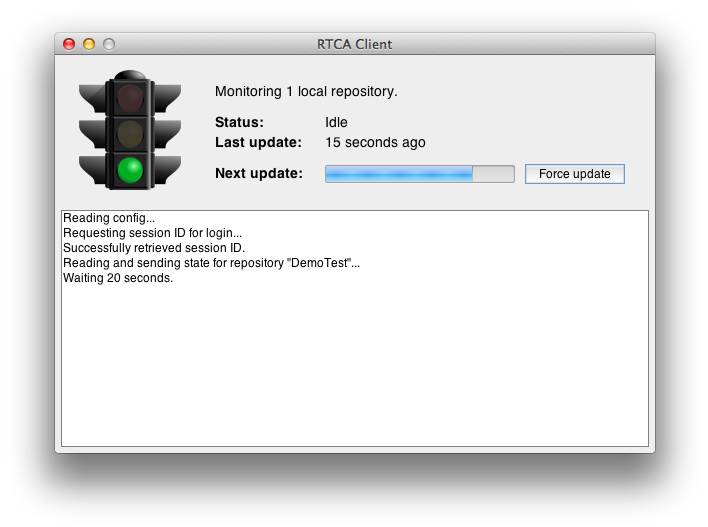
\includegraphics[width=0.8\textwidth]{gui}
  \caption{Screenshot of the CloudStudio client}
  \label{fig:gui}
\end{figure}








\section{Server}

The CloudStudio server is written in Java and is the core of the system. It reads, stores and processes information necessary for awareness requests and conflict detection. There are two main services running on the CloudStudio server: an HTTP server and a service to periodically update information from the central remote Git repositories used by CloudStudio projects. \\

The HTTP server implements the multi-threaded \texttt{com.sun.httpserver} and two separate request handlers deal with API requests and web interface requests on the same port. The class ApiHttpHandler is responsible for calls to URLs prefixed with \texttt{/api/} and provides a public interface for the main CloudStudio server functionality. Any other URLs will be directed to the Web\-Inter\-face\-Http\-Hand\-ler, which is mostly just a static web server; the actual web interface runs in JavaScript and uses the API directly. Details about the implementations of the web interface follow in the next section. \\

PeriodicalAllOriginUpdater is the service to periodically update the remote repository information for all CloudStudio projects. Behind the curtains, it clones the given Git repositories and reads and stores them in the same manner as a regular client would. It uses the special user account "origin", which is added to all projects by default. Table \ref{table:serverclasses} shows an overview of the server's Java classes. The code for all individual classes is commented throughout. For detailed information, have a look at the source code. \\

All CloudStudio data is stored in a MySQL database, accessed either directly through the JDBC driver or using the C3P0 database connection pool, depending on the server settings. \\

The server is greatly customizable through a configuration XML file, described in section \ref{configmanagement}.


\begin{table}

    \scriptsize
    \begin{tabularx}{\textwidth}{ | l | X | }
    \hline
\textbf{Class} & \textbf{Description} \\ \hline
ApiHttpHandler & Handles HTTP exchanges for API requests. \\ \hline
ContentConflictGitReader & Finds the common ancestor needed to find conflicts and do three-way comparisons. \\ \hline
DatabaseConnection & Performs operations on the database. \\ \hline
DatabaseConnctionPool & Accesses and returns a data source from C3P0 database connection pool. \\ \hline
OriginUpdater & Updates remote Git repository information for a single repository and writes information into the database. \\ \hline
PeriodicalAllOriginUpdater & Periodically calls OriginUpdater with all the remote repositories used by CloudStudio projects. \\ \hline
ServerConfig & Reads the configuration file and returns individual parameters. \\ \hline
ServerMain & Main class that reads the config, sets up the origin updater and starts the HTTP server. \\ \hline
SideBySideDiff & Prepares a side-by-side comparison JSON object for two files. \\ \hline
SideBySideThreeWayDiff & Prepares a side-by-side compairson JSON object for a three-way comparison. \\ \hline
SqlQueryReader & Reads and caches SQL queries stored in external files. \\ \hline
WebInterfaceHttpHandler & Handles HTTP requests to the web interface. \\ \hline
ProcessWithTimeout & Helper class to allow a timeout for Process executions. \\ \hline
ParameterFilter & Helper class to parse HTTP GET and POST parameters. \\ \hline
    \end{tabularx}
    
    \centering
  \caption{Server classes}
  \label{table:serverclasses}
\end{table}



\section{Web Interface}

CloudStudio has a web interface that allows you to view awareness information from the browser. The web interface runs on the same server and port as the API. The logic of the web interface runs in JavaScript and on the client side; an approach that is popular with many web services nowadays. The server serves as a static webserver, and awareness data is fetched directly via the CloudStudio API. \\

The CloudStudio web interface uses EJB, a light-weight templating engine, and jQuery, a fast, small, and feature-rich JavaScript library that makes thinks like HTML document manipulation, event handling, and Ajax much simpler. \\

The web interface was designed in a modern way that is user intuitive and easy to understand. The functionality of the web interface is explained in detail in section \ref{webinterfaceguide}.



\section{API}

The CloudStudio API exposes an interface to access and manipulate CloudStudio resources. All CloudStudio resources are accessed and manipulated in a similar way. Requests to the CloudStudio API have to use either the GET or POST method. GET requests are used for functions that do not change the state of the database. POST requests are used for functions that make changes to the database. \\

The content type of requests to the CloudStudio API must be set to \texttt{application/x-www-form-urlencoded}. The response has the content type \texttt{application/json}. This asynchronism allows to provide parameters for both GET and POST requests similarly and still retrieve comprehensive JSON objects, and is used by many widely used APIs (e.g. SoundCloud). The entire API documentation can be found in the Appendix of this thesis or directly on the project's GitHub page.



\section{Database}\label{database}

The back-end for all data stored in the system is a MySQL database. The database is accessed using the JDBC driver directly, or using the C3P0 connection pool framework, depending on the configuration settings. Figure \ref{fig:databasegraph} shows the database tables and their primary (indicated as $PK$) and foreign keys (indicated as arrows). Table \ref{table:databasetables} explains the functionality of each table.


\begin{figure}[h!]
  \centering
      \includegraphics[width=0.8\textwidth]{databasegraph}
  \caption{CloudStudio's database setup}
  \label{fig:databasegraph}
\end{figure}



\begin{table}

    \scriptsize
    \begin{tabularx}{\textwidth}{ | l | X | }
    \hline
\textbf{Table} & \textbf{Functionality} \\ \hline
USERS & Every entry represents a CloudStudio user \\ \hline
REPOSITORIES & Every entry represents a CloudStudio repository \\ \hline
USERSESSION & Every entry represents a session \\ \hline
USERACCESS & Which user has access to a repository (n:n) \\ \hline
BRANCHES & Branches for a user and repository \\ \hline
FILES & Files for a user, repository and branch \\ \hline
COMMITHISTORY & Commit history for a user and repository \\ \hline
    \end{tabularx}
    
    \centering
  \caption{Database tables}
  \label{table:databasetables}
\end{table}



\section{Configuration Management}\label{configmanagement}

\subsection{Client Configuration}

In order to run the client JAR, you need to have a configuration file called \texttt{config.xml} in the same directory. Alternatively, you can also specify the path to a config file as the first parameter. A sample configuration file can be seen in Fig. \ref{fig:clientconfig}. \\

\begin{figure}[h!]
\begin{lstlisting}
 <?xml version="1.0" encoding="UTF-8"?>
 <config>
     <username>John</username>
     <password>burgers</password>
     <serverUrl>http://cloudstudio.ethz.ch:7330</serverUrl>
     <repositories>
         <repository>
             <alias>RepositoryAliasOnCloudStudio</alias>
             <localPath>/path/to/your/local/repository</localPath>
         </repository>
     </repositories>
     <resubmitInterval>300</resubmitInterval>
 </config>
\end{lstlisting}
  \centering
  \caption{Sample client configuration}
  \label{fig:clientconfig}
\end{figure}


Specify your $username$ and $password$ that you previously created for CloudStudio using its API or the web interface. Your user must have been added to the repository on CloudStudio. \\

Under repositories you can list multiple repositories that you want to monitor with CloudStudio. The $repositoryAlias$ is the name that a given repository has on CloudStudio and the $localPath$ is the folder where you locally cloned your Git repository into. Specify a time interval in seconds as the $resubmitInterval$, indicating how often the client sends data to the CloudStudio server.


\subsection{Server Configuration}

Figure \ref{fig:serverconfig} shows a sample configuration. Table \ref{table:serverconfigtable} explains what the individual parameters do. After setting up the configuration file, you need to run \texttt{SQLInit.sql} to initialize the database (MySQL), before starting the server.

\begin{figure}[h!]
\begin{lstlisting}
 <?xml version="1.0" encoding="UTF-8"?>
 <config>
     <serverPort>7330</serverPort>
     <dbDriverClass>com.mysql.jdbc.Driver</dbDriverClass>
     <dbJdbcUrl>jdbc:mysql://localhost/cloudstudio</dbJdbcUrl>
     <dbUser>dbadmin</dbUser>
     <dbPassword>1234</dbPassword>
     <useDatabasePool>true</useDatabasePool>
     <dbMinPoolSize>5</dbMinPoolSize>
     <dbAcquireIncrement>5</dbAcquireIncrement>
     <dbMaxPoolSize>20</dbMaxPoolSize>
     <dbMaxStatements>180</dbMaxStatements>
     <fileStorageDirectory>path/to/filestorage</fileStorageDirectory>
     <originStorageDirectory>path/to/origins</originStorageDirectory>
     <passwordSalt>GXSBML0EGjOMfqPzsznUCkK8ENP3lmOX</passwordSalt>
     <enableOriginUpdate>true</enableOriginUpdate>
     <originUpdateInterval>300</originUpdateInterval>
     <createAdminUser>true</createAdminUser>
     <giveCreatorPrivilegesOnSignUp>true</giveCreatorPrivilegesOnSignUp>
 </config>
\end{lstlisting}
  \centering
  \caption{Sample server configuration}
  \label{fig:serverconfig}
\end{figure}


\begin{table}

    \scriptsize
    \begin{tabularx}{\textwidth}{ | l | X | }
    \hline
\textbf{Setting} & \textbf{Description} \\ \hline
serverPort & Port for the HTTP server hosting the API and the Web Interface \\ \hline
dbDriverClass & JDBC driver \\ \hline
dbJdbcUrl & Database URL \\ \hline
dbUser & Database username \\ \hline
dbPassword & Database password \\ \hline
useDatabasePool & Enable C3P0 database pooling (\emph{true}/\emph{false}) \\ \hline
dbMinPoolSize & C3P0: minimum pool size \\ \hline
dbAcquireIncrement & C3P0: acquire increment \\ \hline
dbMaxPoolSize & C3P0: maximum pool size \\ \hline
dbMaxStatements & C3P0: maximum database statements \\ \hline
fileStorageDirectory & The database only stores file hashes. The file contents to the hashes are stored in this directory. \\ \hline
originStorageDirectory & A clone of the remote repository is stored in this directory for all projects. \\ \hline
passwordSalt & Salt for the password hash \\ \hline
enableOriginUpdate & Periodically fetch all remote repositories (\emph{true}/\emph{false}) \\ \hline
originUpdateInterval & How often to update remote repositories (in seconds) \\ \hline
createAdminUser & Create an administrator with username "Admin" and password "1234" if it doesn't exist on server start (\emph{true}/\emph{false})  \\ \hline
giveCreatorPrivilegesOnSignUp & Automatically give repository creation privileges when a new user is created (\emph{true}/\emph{false})  \\ \hline
    \end{tabularx}
    
    \centering
    
  \caption{Server configuration parameters}
  \label{table:serverconfigtable}
  
    \end{table}
    



\section{Testing and Correctness}

The Eclipse plugin EclEmma \cite{eclemma} was used to create coverage reports and view the line coverage directly in the workbench. EclEmma is a free code coverage tool, based on the JaCoCo library. A high code coverage indicates that the code has been more thoroughly tested and there is a lower chance of software bugs than in a program with low code coverage \cite{codecoverage}. The coverage report created by EclEmma can be seen in Figure \ref{fig:testcoverage}. \\

To verify CloudStudio's correctness, I implemented two different types of JUnit \cite{junit} tests: $class$ $tests$ for client and server verify the correct behaviour for a given class and are named after the class that is being tested, e.g. ApiHttpHandlerTest for ApiHttpHandler; $combination$ $tests$ run longer scenarios of a typical CloudStudio workflow and assert correct behaviour throughout. \\

The CloudStudio client and server use the Apache Log4j \cite{log4j} framework to create log output; it can be customised by editing the \texttt{log4j.xml} file. Log files can as well be used to view and ensure the correct behaviour of the code.


\begin{figure}[h!]
  \centering
      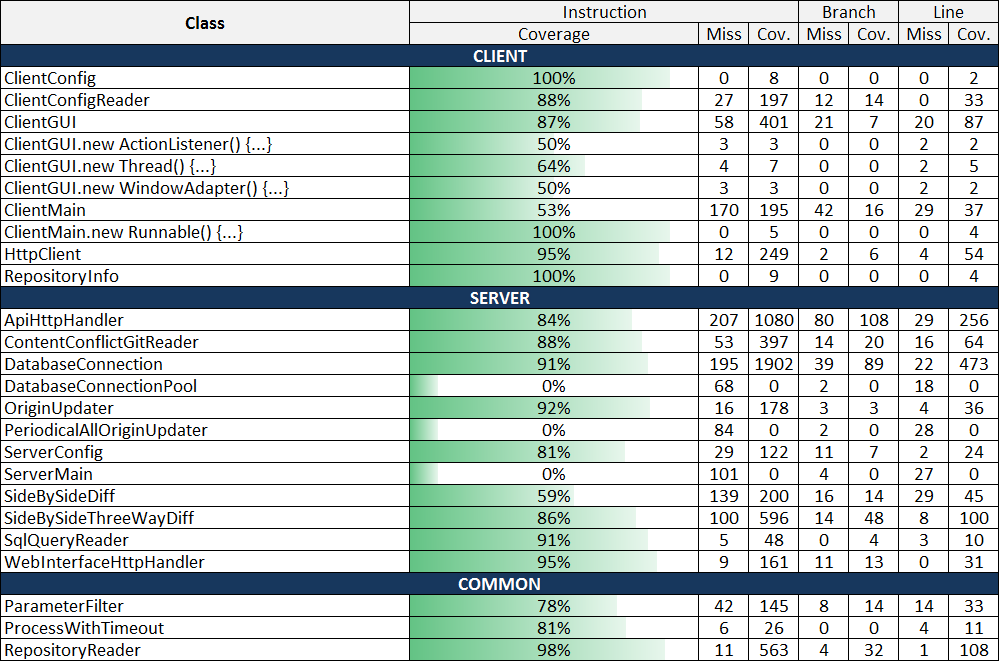
\includegraphics[width=0.9\textwidth]{coverage}
  \caption{Test coverage using EclEmma}
  \label{fig:testcoverage}
\end{figure}



\section{Build and Run}

Follow the following steps to build the CloudStudio server and client locally:

\begin{enumerate}


\item \emph{Clone the project.} \newline
\texttt{git clone https://github.com/fgremper/CloudStudio.git}
\item \emph{Import into Eclipse.} \newline Import the 4 folders CSClient, CSServer, CSCommon and CSTesting as existing Eclipse projects. (Open Eclipse and go to $File$ $\rightarrow$ $Import$ and select $Existing$ $Projects$ $into$ $Workspace$.)
\item \emph{Build JAR} \newline
In Eclipse, go to $File$ $\rightarrow$ $Export$ $\rightarrow$ $Java$ $\rightarrow$ $Runnable$ $JAR$ $file$.
Under $Launch$ $configuration$, select ClientMain to build the client JAR. To build the server JAR, select ServerMain. Under $Library$ $handling$, select $Package$ $required$ $libraries$ $into$ $generated$ $JAR$.
Select the export destination and click Finish.
\item \emph{Run} \newline
Run the client:
\texttt{java -jar CSClient.jar} \newline
Run the server:
\texttt{java -jar CSServer.jar}

\end{enumerate}
